% ============================================================
\chapter{Introduction \`a la Programmation}
\label{ch:intro}
% ============================================================

\section{Pourquoi programmer ?}

\begin{intuition}
Un programme informatique est une \textbf{recette de cuisine} pour l'ordinateur. Tout comme une recette d\'ecrit \'etape par \'etape comment pr\'eparer un plat, un programme d\'ecrit \'etape par \'etape comment r\'esoudre un probl\`eme.
\end{intuition}

En sciences, programmer permet de :
\begin{itemize}
\item \textbf{Automatiser} des calculs r\'ep\'etitifs (calculer 10\,000 int\'egrales).
\item \textbf{Visualiser} des donn\'ees (tracer l'\'evolution d'une population).
\item \textbf{Simuler} des ph\'enom\`enes (mouvement d'un pendule, diffusion de chaleur).
\item \textbf{Analyser} de grandes quantit\'es de donn\'ees (g\'enomique, astronomie).
\end{itemize}

\section{Pourquoi Python ?}

\index{Python}

\begin{center}
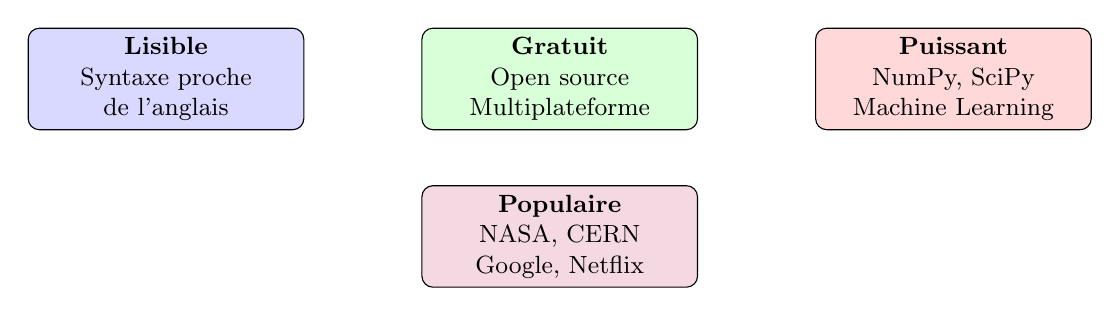
\begin{tikzpicture}[
  box/.style={rectangle, draw, fill=#1!15, rounded corners,
    minimum width=3.5cm, minimum height=0.8cm, align=center, font=\small}
]
\node[box=blue] at (0,0) {\textbf{Lisible}\\Syntaxe proche\\de l'anglais};
\node[box=green] at (5,0) {\textbf{Gratuit}\\Open source\\Multiplateforme};
\node[box=red] at (10,0) {\textbf{Puissant}\\NumPy, SciPy\\Machine Learning};
\node[box=purple] at (5,-2) {\textbf{Populaire}\\NASA, CERN\\Google, Netflix};
\end{tikzpicture}
\end{center}

\section{Votre premier programme}

\begin{codeblock}[title=\textbf{Python}]
\begin{minted}{python}
print("Bonjour, futur(e) scientifique !")
\end{minted}
\end{codeblock}

\begin{codeoutput}
\begin{verbatim}
Bonjour, futur(e) scientifique !
\end{verbatim}
\end{codeoutput}

F\'elicitations ! Vous venez d'\'ecrire votre premier programme. La fonction \py{print()}\index{print} affiche du texte \`a l'\'ecran.

\section{Python comme calculatrice}

Python peut effectuer toutes les op\'erations math\'ematiques de base :

\begin{codeblock}[title=\textbf{Python --- Calculs de base}]
\begin{minted}{python}
# Addition et soustraction
print(3 + 5)
print(10 - 4)

# Multiplication et division
print(6 * 7)
print(15 / 4)     # Division réelle
print(15 // 4)    # Division entière
print(15 % 4)     # Reste (modulo)

# Puissance
print(2 ** 10)     # 2 puissance 10
\end{minted}
\end{codeblock}

\begin{codeoutput}
\begin{verbatim}
8
6
42
3.75
3
3
1024
\end{verbatim}
\end{codeoutput}

\begin{formules}[title=\textbf{Op\'erateurs arithm\'etiques}]
\begin{tabular}{lll}
\toprule
\textbf{Op\'erateur} & \textbf{Signification} & \textbf{Exemple} \\
\midrule
\py{+} & Addition & \py{3 + 5} $= 8$ \\
\py{-} & Soustraction & \py{10 - 4} $= 6$ \\
\py{*} & Multiplication & \py{6 * 7} $= 42$ \\
\py{/} & Division r\'eelle & \py{15 / 4} $= 3.75$ \\
\py{//} & Division enti\`ere & \py{15 // 4} $= 3$ \\
\py{\%} & Modulo (reste) & \py{15 \% 4} $= 3$ \\
\py{**} & Puissance & \py{2 ** 10} $= 1024$ \\
\bottomrule
\end{tabular}
\end{formules}

\section{Commentaires}

Les \textbf{commentaires}\index{commentaire} sont des notes pour les humains. Python les ignore compl\`etement.

\begin{codeblock}[title=\textbf{Python}]
\begin{minted}{python}
# Ceci est un commentaire — Python l'ignore
print(2 + 3)   # On peut commenter en fin de ligne

# Vitesse de la lumière en m/s
c = 299792458
print(f"Vitesse de la lumière : {c} m/s")
\end{minted}
\end{codeblock}

\begin{codeoutput}
\begin{verbatim}
5
Vitesse de la lumière : 299792458 m/s
\end{verbatim}
\end{codeoutput}

\begin{bonnepratique}
Commentez votre code pour expliquer \textbf{pourquoi} vous faites quelque chose, pas \textbf{ce que} vous faites. Un bon commentaire dit <<~Vitesse de la lumi\`ere en m/s~>>, pas <<~On affecte 299792458 \`a c~>>.
\end{bonnepratique}

\section{Exemple scientifique : \'Energie cin\'etique}

Calculons l'\'energie cin\'etique $E_c = \frac{1}{2}mv^2$ d'un objet :

\begin{codeblock}[title=\textbf{Python --- \'Energie cin\'etique}]
\begin{minted}{python}
# Données
masse = 75.0       # kg (une personne)
vitesse = 10.0     # m/s (course rapide)

# Calcul de l'énergie cinétique
Ec = 0.5 * masse * vitesse ** 2

print(f"Masse    : {masse} kg")
print(f"Vitesse  : {vitesse} m/s")
print(f"Énergie  : {Ec} J")
\end{minted}
\end{codeblock}

\begin{codeoutput}
\begin{verbatim}
Masse    : 75.0 kg
Vitesse  : 10.0 m/s
Énergie  : 3750.0 J
\end{verbatim}
\end{codeoutput}

\section{Les erreurs : ne pas avoir peur !}

\begin{errmark}
Les erreurs sont \textbf{normales} et font partie de l'apprentissage. Python vous aide en indiquant le type d'erreur et la ligne concern\'ee.

\begin{codeblock}[title=\textbf{Python --- Erreurs courantes}]
\begin{minted}{python}
# Erreur de syntaxe : parenthèse oubliée
# print("Bonjour"
# SyntaxError: '(' was never closed

# Erreur de nom : variable non définie
# print(x)
# NameError: name 'x' is not defined

# Erreur de type : opération impossible
# "abc" + 5
# TypeError: can only concatenate str to str

# Division par zéro
# 10 / 0
# ZeroDivisionError: division by zero
\end{minted}
\end{codeblock}

\textbf{R\`egle d'or} : lisez toujours le message d'erreur \textbf{de bas en haut}. La derni\`ere ligne vous dit ce qui ne va pas.
\end{errmark}

\section{Le mode interactif vs les scripts}

\begin{center}
\begin{tikzpicture}[
  box/.style={rectangle, draw, fill=#1!15, rounded corners,
    minimum width=5cm, minimum height=2cm, align=center, font=\small}
]
\node[box=blue] (inter) at (0,0) {\textbf{Mode interactif}\\(Jupyter, console)\\Tester, explorer\\R\'eponse imm\'ediate};
\node[box=green] (script) at (7,0) {\textbf{Script}\\(fichier .py)\\Programme complet\\R\'eutilisable};
\draw[-{Stealth},thick,dashed] (inter) -- node[above,font=\scriptsize]{Prototyper} node[below,font=\scriptsize]{puis automatiser} (script);
\end{tikzpicture}
\end{center}

\section{Mini-projet : Conversions d'unit\'es}

\begin{projet}
\'Ecrivez un programme qui convertit des temp\'eratures entre Celsius et Fahrenheit.

\textbf{Formules} : $F = \frac{9}{5}C + 32$ et $C = \frac{5}{9}(F - 32)$

\begin{codeblock}[title=\textbf{Python --- Convertisseur}]
\begin{minted}{python}
# Conversion Celsius -> Fahrenheit
celsius = 100
fahrenheit = (9/5) * celsius + 32
print(f"{celsius}°C = {fahrenheit}°F")

# Conversion Fahrenheit -> Celsius
fahrenheit = 72
celsius = (5/9) * (fahrenheit - 32)
print(f"{fahrenheit}°F = {celsius:.1f}°C")

# Table de conversion
print("\n--- Table de conversion ---")
print(f"{'°C':>6}  {'°F':>6}")
for c in range(0, 101, 10):
    f = (9/5) * c + 32
    print(f"{c:>6}  {f:>6.1f}")
\end{minted}
\end{codeblock}

\begin{codeoutput}
\begin{verbatim}
100°C = 212.0°F
72°F = 22.2°C

--- Table de conversion ---
    °C      °F
     0    32.0
    10    50.0
    20    68.0
    30    86.0
    40   104.0
    50   122.0
    60   140.0
    70   158.0
    80   176.0
    90   194.0
   100   212.0
\end{verbatim}
\end{codeoutput}
\end{projet}

\section{Exercices}

\begin{exercice}[$\star$ --- Guid\'e]
Calculez l'aire d'un cercle de rayon $r = 5$ en utilisant la formule $A = \pi r^2$. Utilisez \py{3.14159} pour $\pi$.
\end{exercice}

\begin{exercice}[$\star$ --- Guid\'e]
Calculez la distance entre deux points $(x_1, y_1) = (1, 2)$ et $(x_2, y_2) = (4, 6)$ avec la formule $d = \sqrt{(x_2-x_1)^2 + (y_2-y_1)^2}$. Indice : $\sqrt{x} = x^{0.5}$.
\end{exercice}

\begin{exercice}[$\star\star$ --- Ind\'ependant]
La loi de la gravitation universelle donne la force entre deux masses : $F = G\frac{m_1 m_2}{r^2}$, avec $G = 6.674 \times 10^{-11}$~N$\cdot$m$^2$/kg$^2$. Calculez la force entre la Terre ($m_1 = 5.972 \times 10^{24}$~kg) et la Lune ($m_2 = 7.342 \times 10^{22}$~kg), distantes de $r = 3.844 \times 10^{8}$~m.
\end{exercice}

\begin{exercice}[$\star\star\star$ --- D\'efi scientifique]
Calculez la longueur d'onde de De Broglie $\lambda = h / (mv)$ pour un \'electron ($m = 9.109 \times 10^{-31}$~kg) se d\'epla\c{c}ant \`a $v = 10^6$~m/s, avec $h = 6.626 \times 10^{-34}$~J$\cdot$s. Comparez avec la taille d'un atome ($\sim 10^{-10}$~m).
\end{exercice}

\begin{formules}[title=\textbf{R\'esum\'e du chapitre}]
\begin{itemize}
\item \py{print()} affiche du texte et des valeurs.
\item Python conna\^it les op\'erations : \py{+}, \py{-}, \py{*}, \py{/}, \py{//}, \py{\%}, \py{**}.
\item Les commentaires commencent par \py{#}.
\item Les erreurs sont normales --- lisez le message de bas en haut.
\item Un script \py{.py} est un programme r\'eutilisable.
\end{itemize}
\end{formules}
